%----------------------------------------------------------------
%
%  File    :  text-only-browsers.tex
%
%  Author  :  Olli-Pekka Riikola, TU Graz, Austria
% 
%  Created :  2.12.2022
% 
%----------------------------------------------------------------


\chapter{Text-Only Browsers}%
\label{ch:tb}

Originally, text browsers were the only way to browse the web. Also,
back in the days, internet connection speeds used to be much slower
than today but similarly, websites were much simpler and it was
possible to access them even with the narrow bandwidth. After
that there are now several powerful graphical web browsers for web
users, but the text browsers still have some important use cases even
they are quite an old solution for web browsing
\parencite{best-text-browsers}. In addition, there are still a few
promising text browser remaining and even receiving recent updates at
least annually, and they are worth having a look.


\section{Text-Only Browsers in Use}%
\label{sec:tb-known}

The header above might seems to be a bit exaggerated, but it is
possible and sensible to use text browsers on a daily
basis. This is because text browsers are lightweight software and
still efficient on poor internet connection and they could actually
help users to reduce distraction while browsing the web and that is why
they could be a good choice for a browser even nowadays. The text
browsers are designed to logically organize the content of the website
rather than just be ordinary web browsers that give access to
the site to a user. More than that, persons with no sight or who are
partially impaired can more efficiently access a website with a text
browser in combination with a screen reader. And when talking about
blind persons as web users it is important to consider, that they
obviously can't see or otherwise access the actual graphical pieces of
art, images, videos, or other similar media formats on the
website \parencite[Chapter 2]{webbie}. So, text browsers reduce the
content that screen readers cannot read and that way they will make
web browsing more convenient for blind people.


\section{Common Problems}%
\label{sec:tb-problems}

Even though the layout of the site would be simple in a text browser, it still
is not simple in practice. According to \textcite[Chapter 5]{webbie} the
reason is presentation. People with sight can have the advantage of a very
versatile navigation link list, but for a blind user, it might be a
struggle. It becomes a struggle at the point when the text browser tries to
present the navigation bar as a list of links, and the screen reader starts to
read it --- link by link, one by one. Luckily, there is an option to
skip this navigation bar and go straight to the content, but only if
the element is designed properly on the website. Otherwise, the text
browser does not realize that there is a navigation bar, but it just
presents it like a list of links and the user needs to handle it.

Another issue is empty attributes of an element, like the ALT attribute in
IMAGE element. And of course, this problem would quite easily be fixed
by the programmer, especially with powerful accessibility checking
tools, but sadly it is not always like that. So, since images are not
relevant content for a person with no sight, it is very important that
the ALT tag will tell, what is going on in that part of the
website. Also, if an image is for hyperlink, then it should also tell
with ALT tag, where it will bring the user \parencite[Chapter 5]{webbie}.

Perhaps, the most difficult issue in the terms of text browsers is
dynamic content. Since most text browsers do not support JavaScript,
some functionality is not available for the user on the site. This
essentially means that text browsers are not so convenient
way to browse the web anymore. But still, as mentioned before,
there are few interesting text browser software available on the
internet.


\section{Known Text-Only Browsers}%
\label{sec:tb-browsers}

There are several surprisingly well-working text browsers available 
in the internet. Even though there are those powerful and good looking 
graphical browsers too, text browsers have been kept up to date 
and they can be used for browsing todays websites. Of course, 
as mentioned in Section~\ref{sec:tb-problems}, if the design 
of a website is poor, it will not perform very well when accessed 
via the text browser. But what text browsers can be used then, 
the following sections will answer for that.


\subsection{Lynx}%
\label{subsec:tb-lynx}

Lynx is quite an old text browser and it appears to be probably the 
most well-known one. But as it is in the \textcite{lynx} website, Lynx is a
command line interface WWW client for Unix systems. An interesting
side note could also be, that years ago Lynx has been a
solution to build Campus Wide Information Systems.


\subsection{WebbIE}%
\label{subsec:tb-webbie}

WebbIE is one which is designed to help visually impaired persons
to access the web. They are dedicated to work in combination with
screenreaders, like JAWS, WindowEyes, Thunder, NVDA, and Narrator as
mentioned in the \textcite{webbie-main} website. WebbIE runs on
Windows, and it seems to be pretty much the only choice for Windows users.


\subsection{W3M}%
\label{subsec:tb-w3m}

W3M is also a very handy text browser and it works as a pager too, like
`more' or `less' as it says in \textcite{w3m} website. It also works
as a text formatting tool from HTML to plain text.


\subsection{Links}%
\label{subsec:tb-links}

Another interesting and very nicely working text browser is Links
which is a school project from the days in 1999. But since then it has
been kept up to date and many people are involved in the project and
put effort to make Links more diverse \parencite{links}. It runs on
Unix.


\subsection{Others}%
\label{subsec:tb-others}

There are also a few cases worth mentioning, perhaps even if they are not
in the same class as those mentioned above. However, there is a
project called Browsh, which is a graphical text browser running on
Linux. It supports JavaScript, so all functionality in the site should
be accessed but it is still a very early stage of development. But
it might be useful on a poor internet connection.

Other ones are more like plugins, but it is good to know, that there
is such available. Chrome offers a plugin, which makes a website like a text
site, but it seems to be somehow outdated and poor. A more interesting
and very well-working built-in function is Firefox Reader View. It
just makes the website to be easier to read by removing distracting
elements and making the content to be more clearly seen. This function
can be activated just by pressing F9 in the Firefox browser and it
works on several websites.

Additionally, in the paper there are images presenting how powerful text browsers actually could
be. In the case of mirror.co.uk, even if there is plenty of images and
advertisements, the text browsers are able to present the content
somehow sensible as shown in the image~ref{fig:lynx-mirror}. 
There are no images presented from other text browsers, since most 
interesting examples are Lynx and
WebbIE.~Others are more or less similar than the Lynx --- only thing to
consider is, that only W3M and Links work responsively inside of CLI, Lynx
does not.

Also, there is provided interesting data about these text browsers 
in the form of a simple table. Due to the simplicity of the text
browsers, it is easy to get familiar with them by only watching a
showcase video introduced in the Section~\ref{sec:tb-showcase} and 
comparing the screenshots mentioned earlier. But the Table~\ref{tab:text-browsers-info} 
gives a good overview of the text browsers.


% It is preferred to place the table just after this section, used [htp]
\begin{table}[htp]
\tablestretch%
\rowcolors{2}{}{tablerowcolour}
\centering
\begin{tabularx}{\linewidth}
{>{\kern-\tabcolsep}llXX<{\kern-\tabcolsep}}
\toprule
\textbf{Browser} & \textbf{Last update} & \textbf{System} & \textbf{Licence} \\
\midrule
Lynx & 2020, Feb, 27 (v2.9.0) & Linux & Free \\
%
WebbIE & 2021, Dec, 23 (v5.1.0) & Windows & Free \\
%
W3M & 2022, Sep, 17 (v2.28) & Linux & Free \\
%
Links & 2022, Sep, 17 (v2.28) & Linux & Free \\
%
\bottomrule
\end{tabularx}

\caption[Text-Only Browser Information]
{
Information of text browsers
}%
\label{tab:text-browsers-info}
\end{table}


\begin{figure}[tp]
\centering
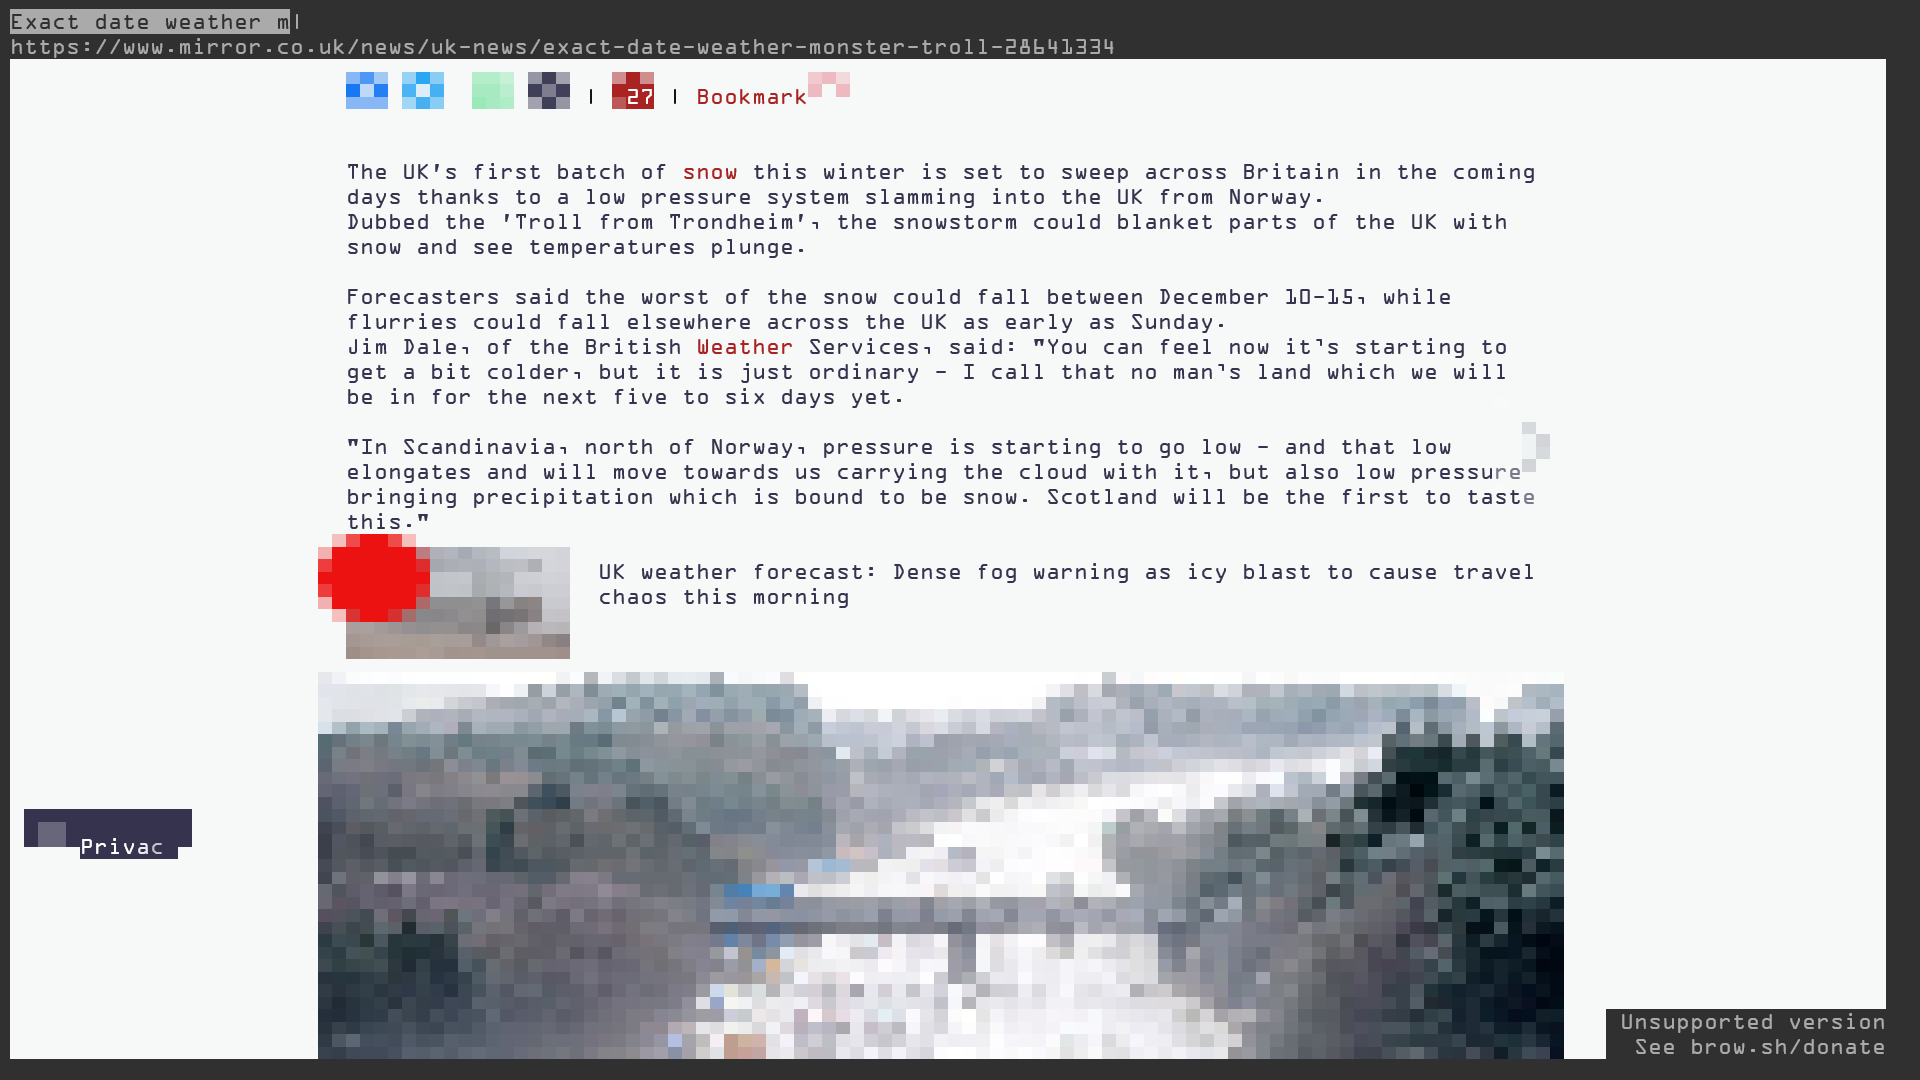
\includegraphics[keepaspectratio,width=\linewidth,height=\halfh]
{images/browsh.png}

\caption[Browsh Graphical CLI Browser]
{%
Browsing the web with Browsh in website gov.uk.
}%
\label{fig:browsh}
\end{figure}


\begin{figure}[tp]
\centering
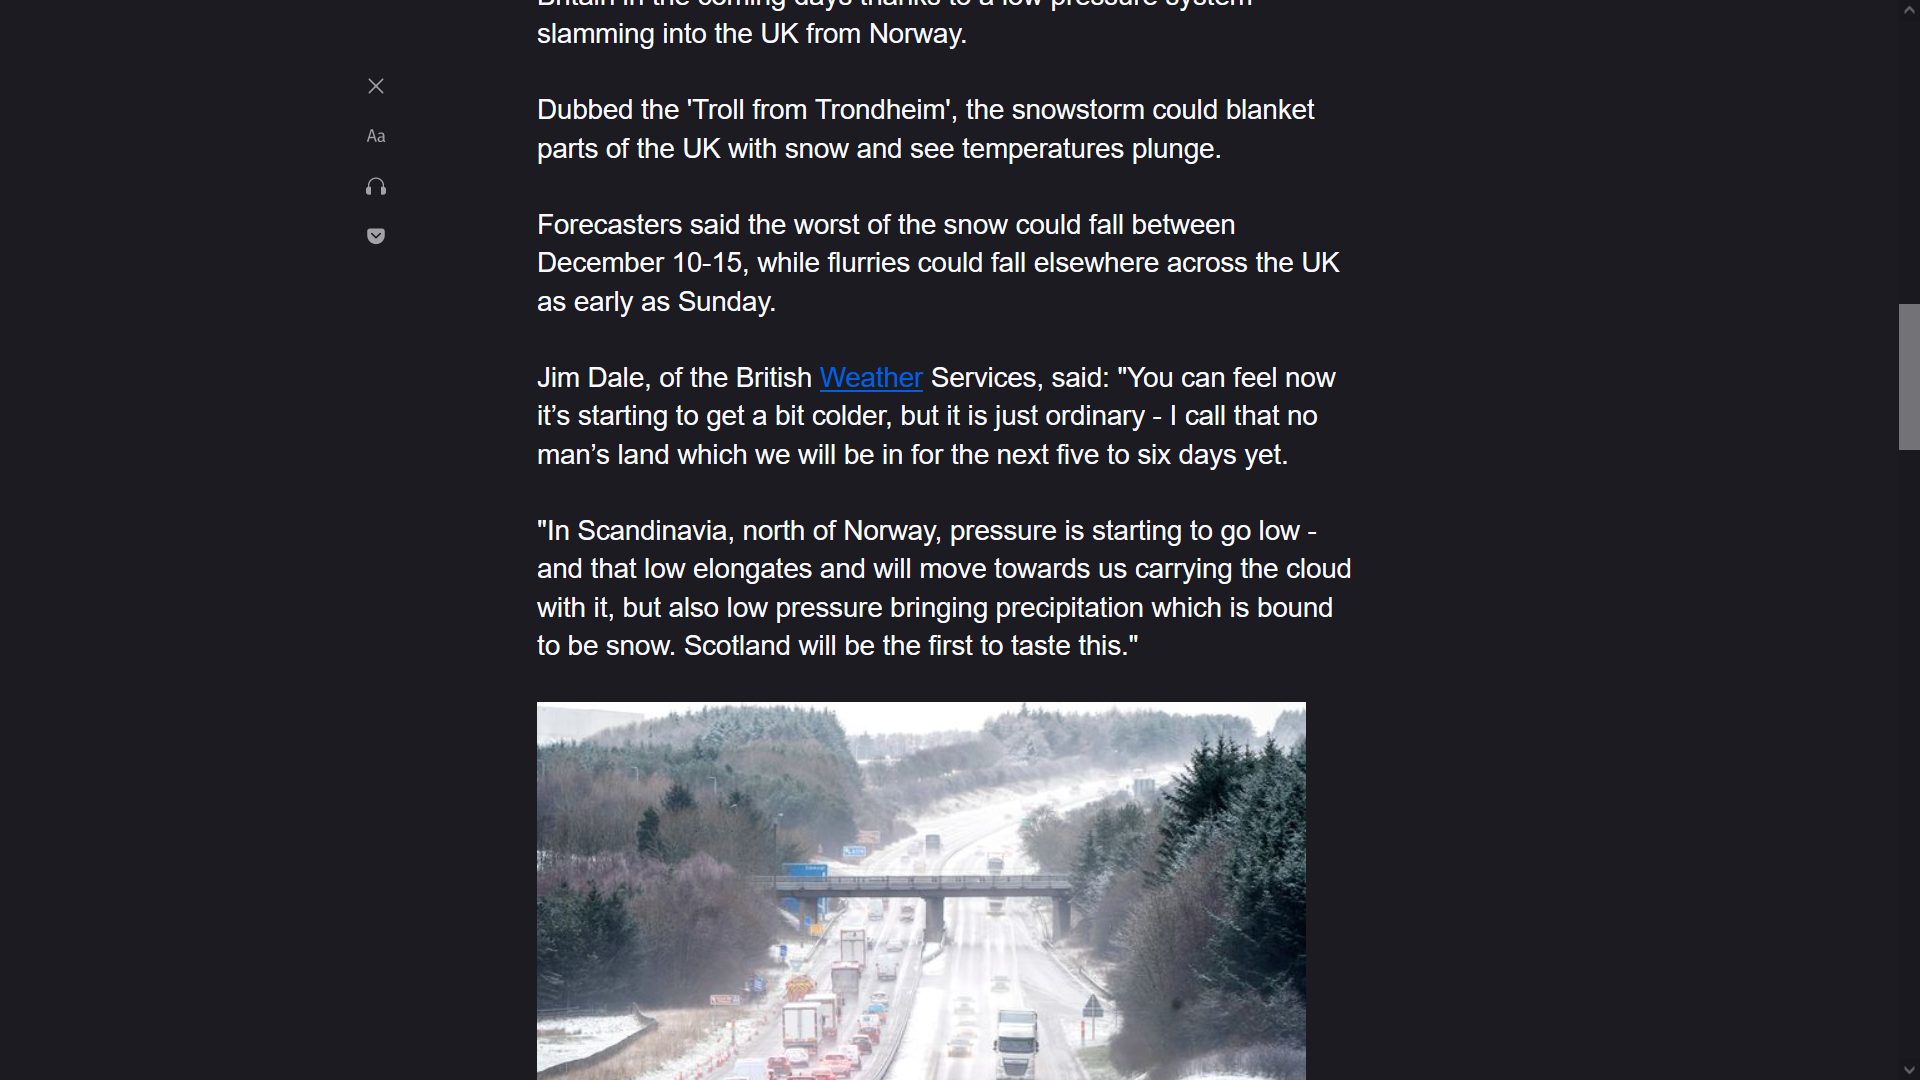
\includegraphics[keepaspectratio,width=\linewidth,height=\halfh]
{images/reader-view.png}

\caption[Firefox Reader View]
{%
Firefox Reader View makes content easier to read.
}%
\label{fig:firefox-rv}
\end{figure}


\section{Showcase Videos}%
\label{sec:tb-showcase}

There is a showcase video on YouTube, where is shown what it looks
like when browsing the web with the Lynx text browser. In the video, it
is shown two examples, gov.uk and mirror.co.uk, which represent 
examples of good and bad web accessibility. Both videos are quite
similar in structure, just tabbing through the sites and entering the
links, but that way it is easy to recognize the problems at the first
glance on the mirror.co.uk website. Link to the showcase video is 
among the references and it is named as \textcite{tb-showcase}.


%\section{Screenshots and Basic Information}%
%\label{sec:tb-screenshots}


\section{Text-Only Browsers Conclusion}

Text Browsers are a handy way to access the web with simple 
interface and they also help to check the web accessibility 
in the current website. Meanwhile the other text browsers just 
concentrate on providing lightweight and simple experiments of 
web browsing, WebbIE is more dedicated to blind users and it is 
very convenient to use in combination with a screen reader. Text 
browsers are not really in daily use nowadays and they are not very 
useful in today's dynamic web content, but still they are quite 
recently updated and they offer a non-distracting way to read 
content on the web. And even better, it is not really necessary to 
install a text browser at all, since Mozilla Firefox browser provides the 
its own built-in Reader View, which is a very convenient way to simplify 
the layout of the current website.


\begin{figure}[tp]
\centering
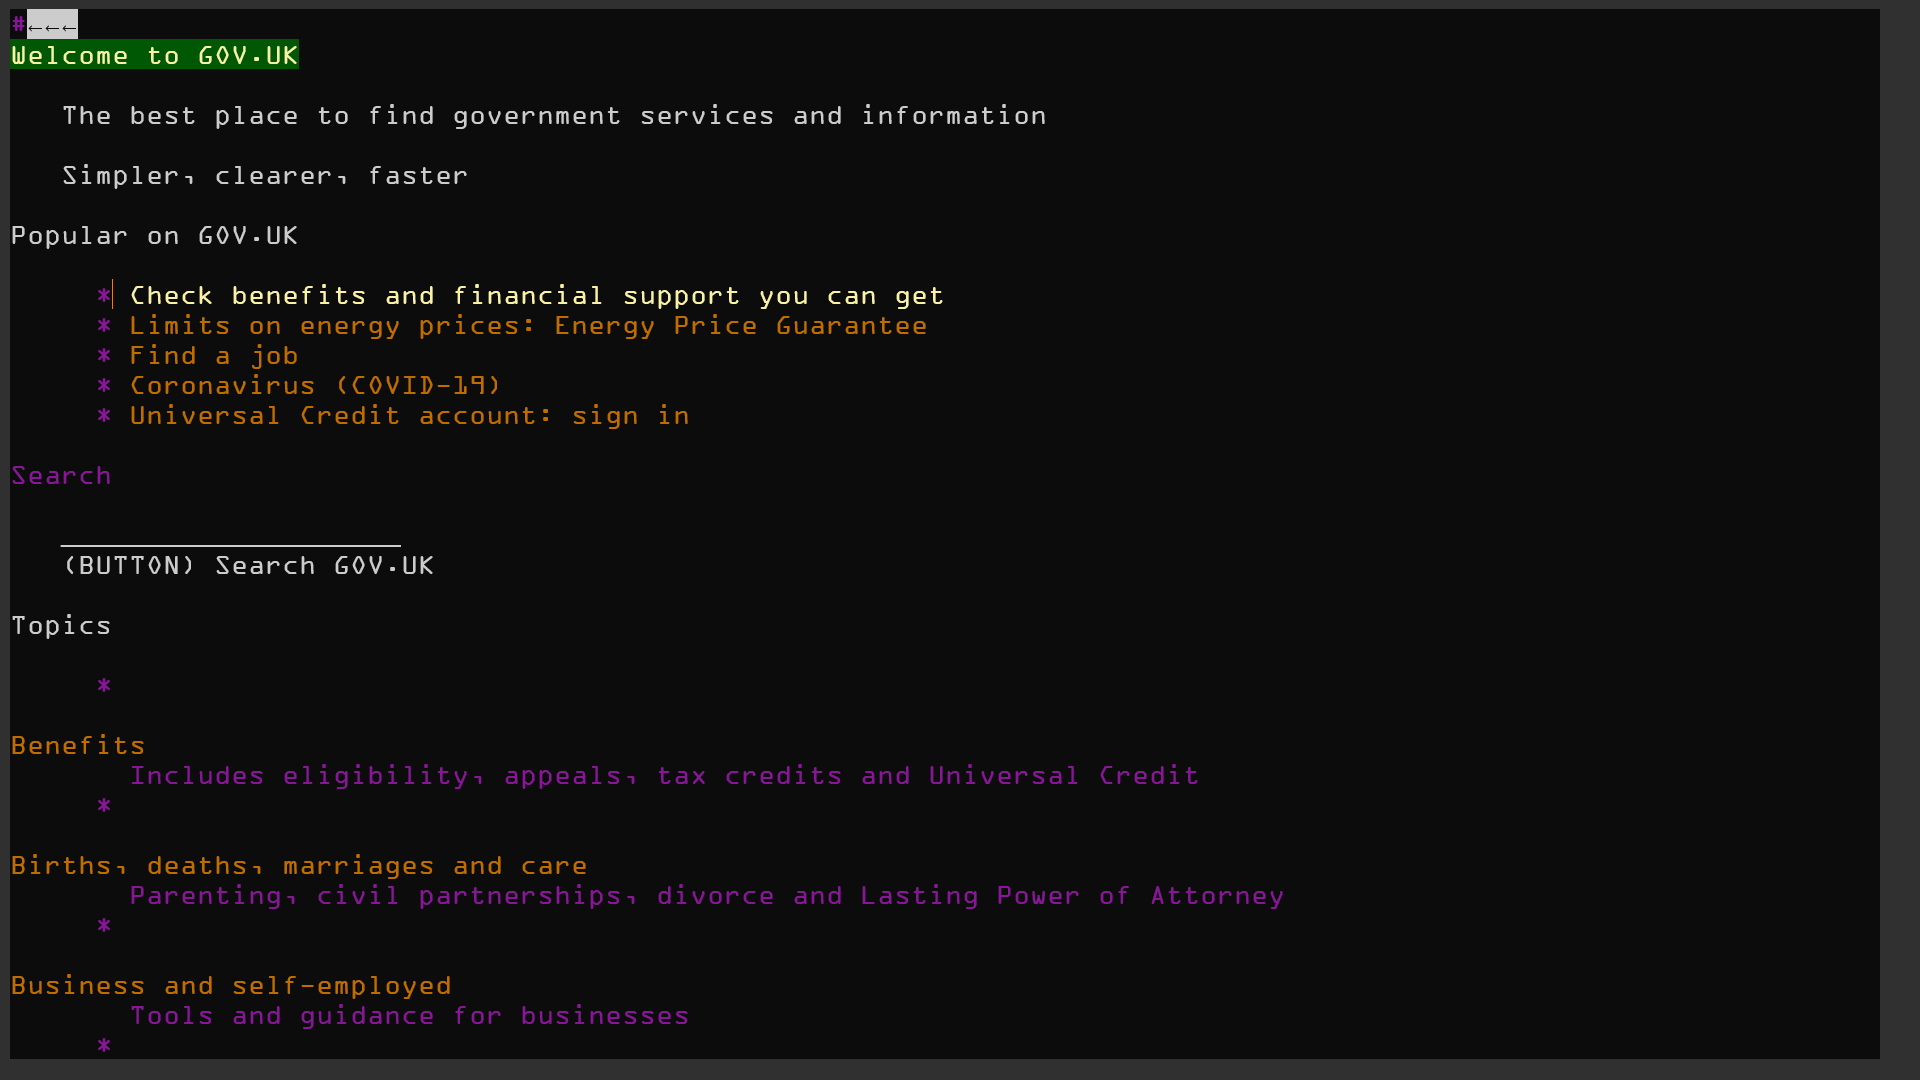
\includegraphics[keepaspectratio,width=\linewidth]
{images/lynx-gov}

\caption[Lynx Browser]
{%
Browsing the gov.uk website
}%
\label{fig:lynx-gov}
\end{figure}


\begin{figure}
\centering
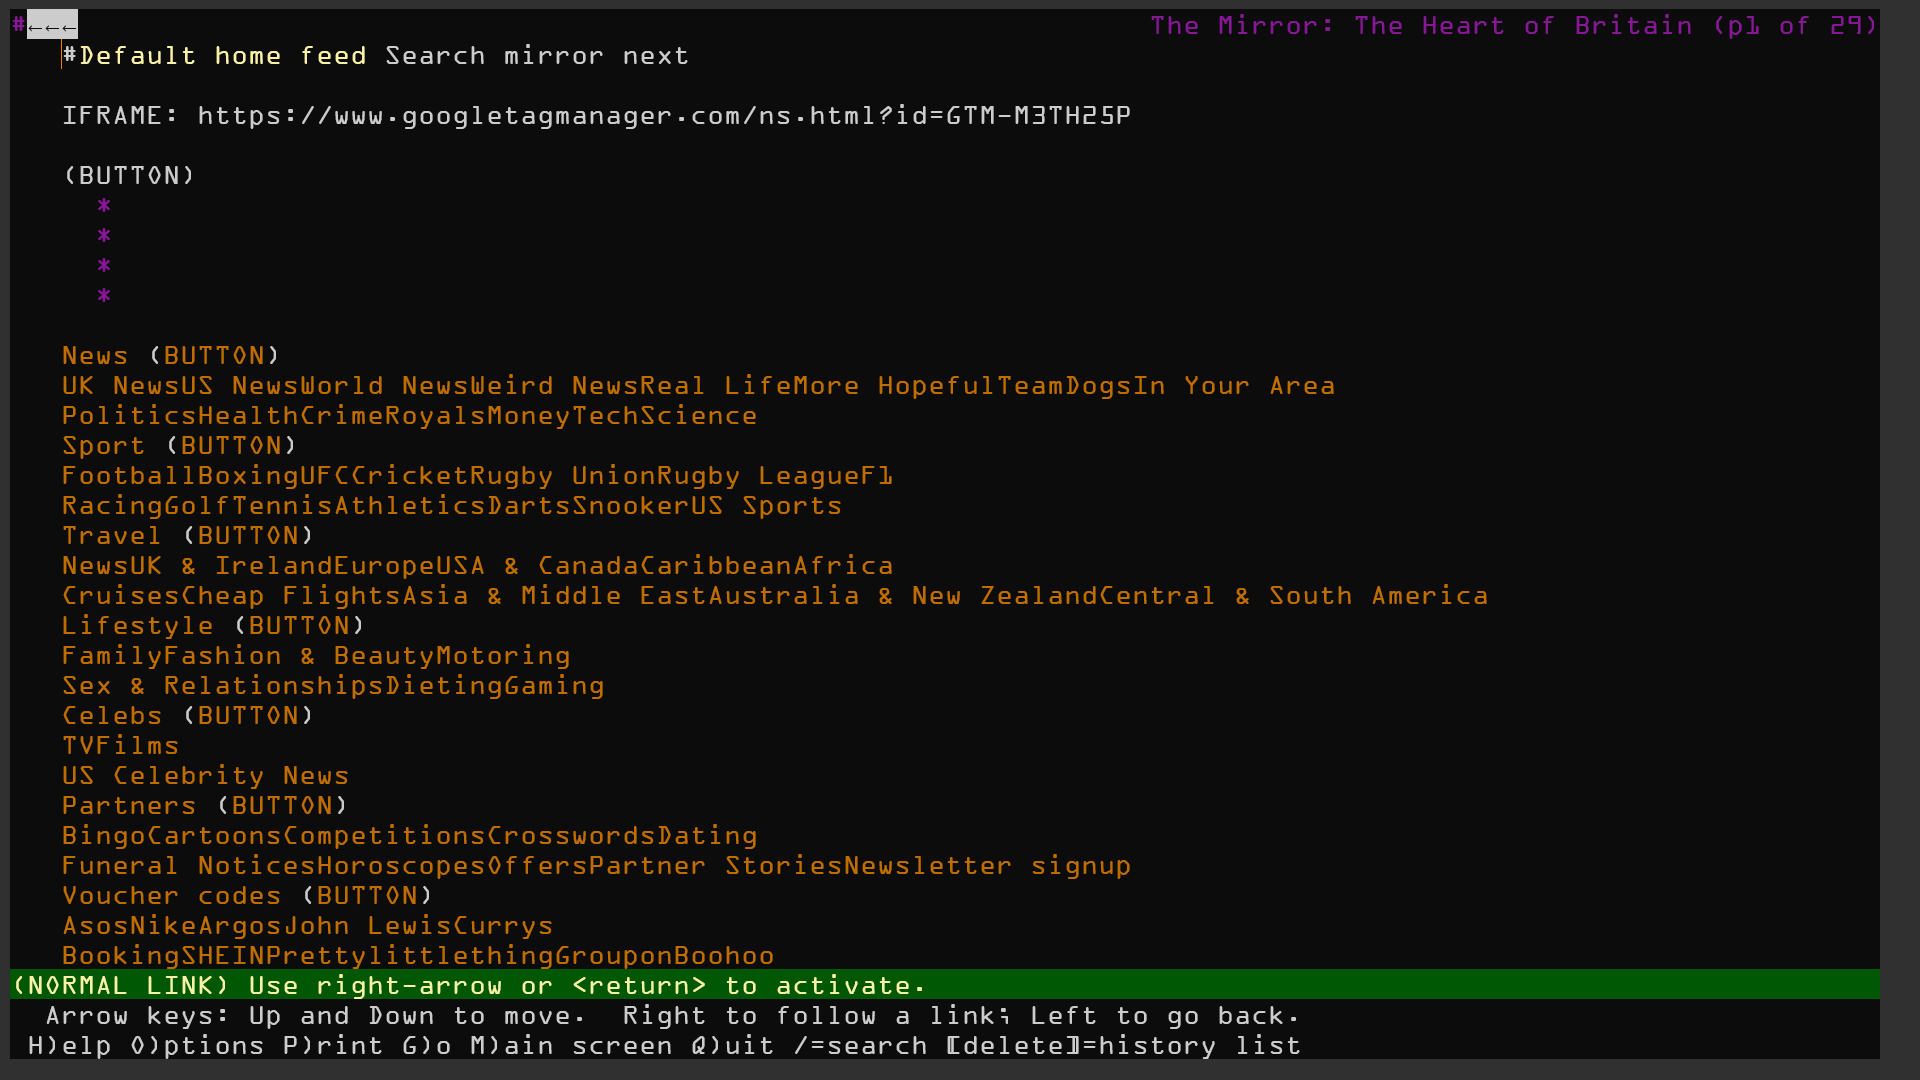
\includegraphics[keepaspectratio,width=\linewidth]
{images/lynx-mirror}

\caption[Lynx Browser]
{%
Browsing the mirror.co.uk website
}%
\label{fig:lynx-mirror}
\end{figure}


\begin{figure}[tp]
\centering
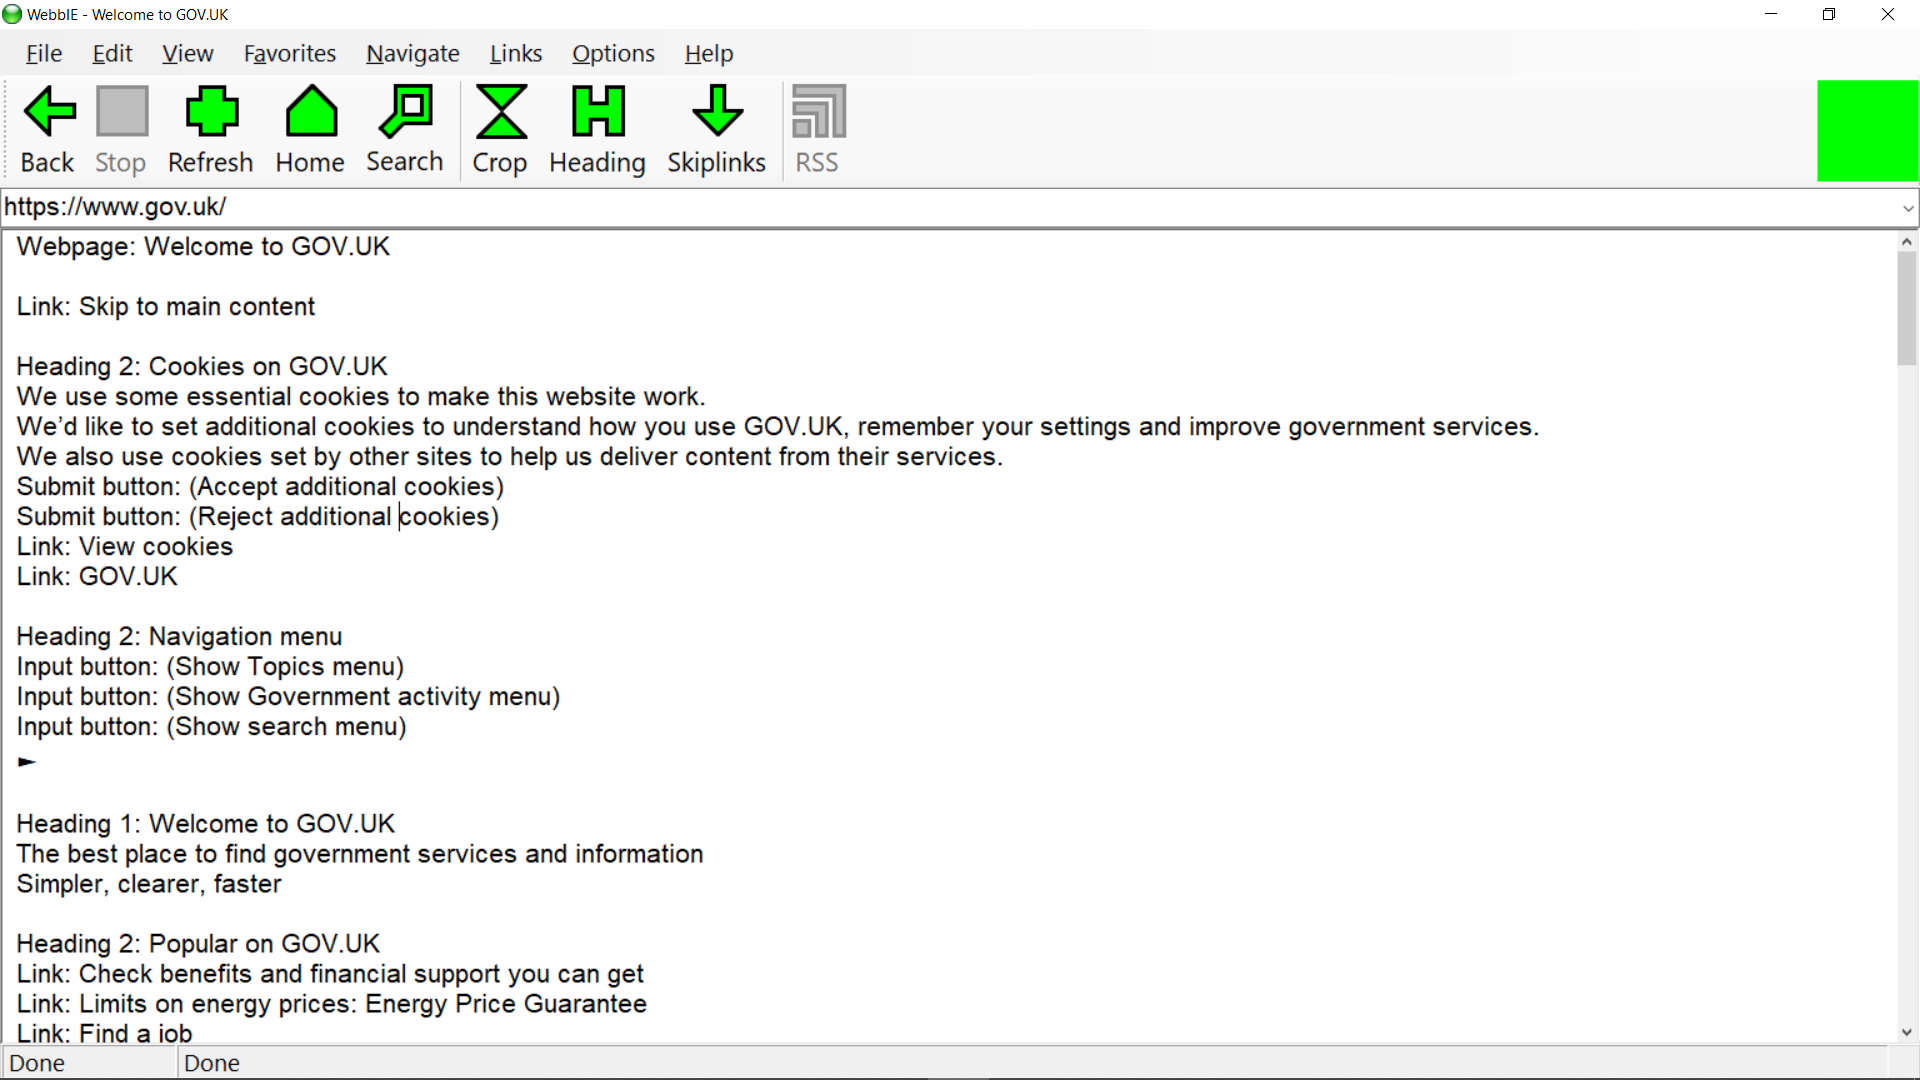
\includegraphics[keepaspectratio,width=\linewidth]
{images/webbie-gov}

\caption[WebbIE Browser]
{%
Browsing the gov.uk website
}%
\label{fig:webbie-gov}
\end{figure}


\begin{figure}
\centering
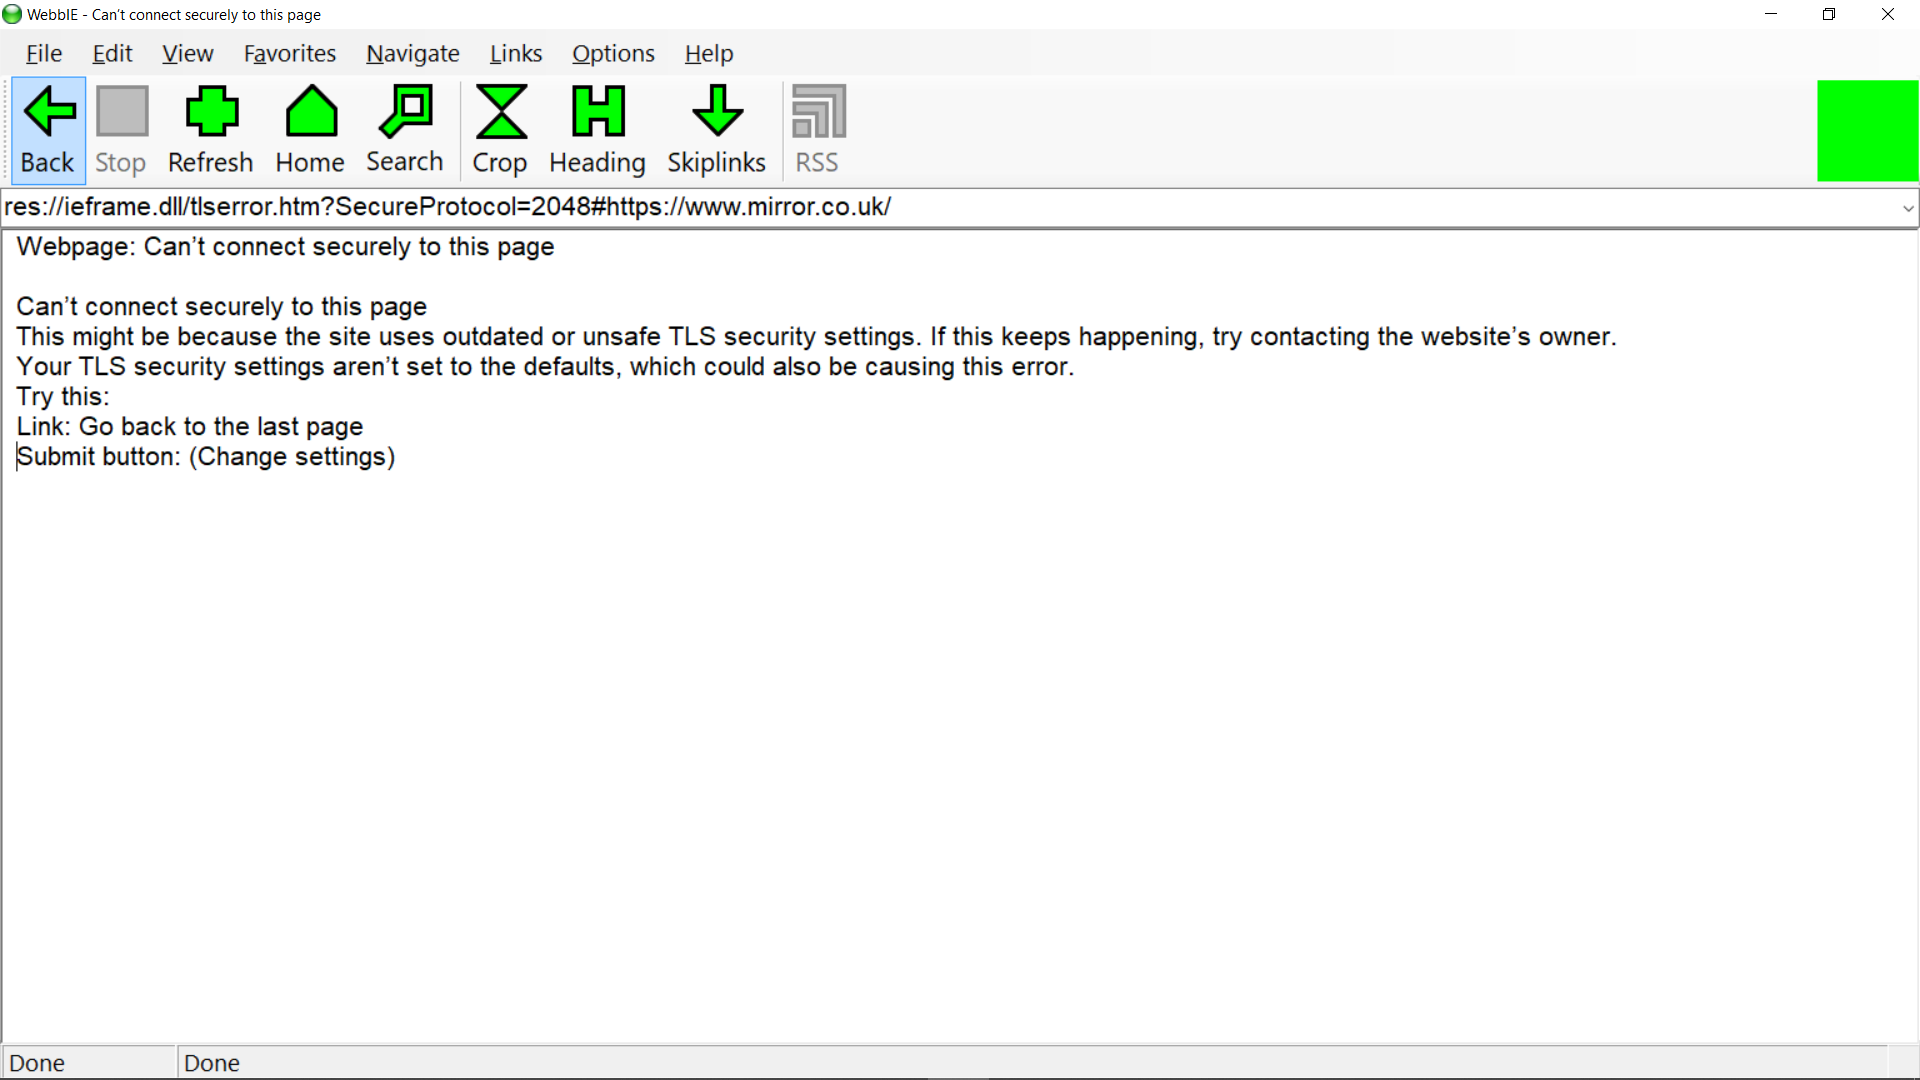
\includegraphics[keepaspectratio,width=\linewidth]
{images/webbie-mirror}

\caption[WebbIE Browser]
{%
Browsing the mirror.co.uk website
}%
\label{fig:webbie-mirror}
\end{figure}
